%----------------------------------------------------------------------------------------
%	PAQUETES Y CONFIGURACION GENERAL
%----------------------------------------------------------------------------------------

\documentclass{article}

% ---- Entrada y salida de texto -----
\usepackage[utf8]{inputenc}

% ---- Márgenes ------
\usepackage[margin=1.3in]{geometry}

% ---- Idioma --------
\usepackage[spanish, es-tabla]{babel} % Selecciona el español para palabras introducidas automáticamente, p.ej. "septiembre" en la fecha y especifica que se use la palabra Tabla en vez de Cuadro

% ------ Requerido para tablas
\usepackage{graphicx}
\usepackage[table,xcdraw]{xcolor}
\usepackage{colortbl} % permite añadir colores a tablas
\usepackage{multirow} % para hacer tablas complejas
\usepackage{threeparttable}



% ---- Otros paquetes ----
\RequirePackage{verbatim}

% para que aparezcan las referencias en el índice de contenido.
\usepackage[nottoc,numbib]{tocbibind}

\usepackage[scaled]{beramono} % escala la fuente de texttt con respecto a la fuente del texto

\usepackage{hyperref} % utilizado para que el indice tenga hipervinculos.
\hypersetup{
    colorlinks,
    citecolor=black,
    filecolor=black,
    linkcolor=black,
    urlcolor=black
} % elimina los bordes rojos un poco molestos de hyperref
\usepackage{url} % ,href} %para incluir URLs e hipervínculos dentro del texto (aunque hay que instalar href)
\usepackage{amsmath,amsfonts,amsthm} % Math packages
%\usepackage{graphics,graphicx, floatrow} %para incluir imágenes y notas en las imágenes
\usepackage{graphics,graphicx, float} %para incluir imágenes y colocarlas

\usepackage{fancyvrb}
%\usepackage{sectsty} % Allows customizing section commands
%\allsectionsfont{\centering \normalfont\scshape} % Make all sections centered, the default font and small caps

\usepackage{fancyhdr} % Custom headers and footers
\pagestyle{fancyplain} % Makes all pages in the document conform to the custom headers and footers
\fancyhead{} % No page header - if you want one, create it in the same way as the footers below
\fancyfoot[L]{} % Empty left footer
\fancyfoot[C]{} % Empty center footer
\fancyfoot[R]{\thepage} % Page numbering for right footer
\renewcommand{\headrulewidth}{0pt} % Remove header underlines
\renewcommand{\footrulewidth}{0pt} % Remove footer underlines
\setlength{\headheight}{13.6pt} % Customize the height of the header
\setlength\parindent{0pt} % Removes all indentation from paragraphs - comment this line for an assignment with lots of text

\newcommand{\horrule}[1]{\rule{\linewidth}{#1}} % Create horizontal rule command with 1 argument of height

% minted ofrece resaltado de sintaxis para código
\usepackage{minted}
\definecolor{bg}{rgb}{0.95,0.95,0.95} 
\usepackage{lmodern}

%----------------------------------------------------------------------------------------
%	TÍTULO Y DATOS DE LOS ALUMNOS
%----------------------------------------------------------------------------------------
\title{	
	
\includegraphics[scale=0.8]{escudoUGR}\\ % also works with logo.pdf
	\normalfont \normalsize 
	\textsc{\textbf{Programación Paralela (2019-2020)} \\ Grado en Ingeniería Informática \\ Universidad de Granada} \\ [30pt] % Your university, school and/or department name(s)
	\horrule{0.5pt} \\[0.4cm] % Thin top horizontal rule
	\huge Práctica 1:
	Implementación de algoritmos paralelos
	de datos en GPU usando CUDA\\ % The assignment title
	\horrule{2pt} \\[0.5cm] % Thick bottom horizontal rule
}  

\author{
	Víctor Peralta Cámara\\
}

%----------------------------------------------------------------------------------------
% DOCUMENTO
%----------------------------------------------------------------------------------------
\begin{document}
 
\maketitle
\newpage

\section{Implementación en CUDA del Algoritmo de Floyd}
\subsection{Primera aproximación}
Mi primer código funcional utilizando un grid bidimensional con bloques bidimensionales es el siguiente:

\begin{minted}[bgcolor=bg,showspaces=false,breaklines=true,tabsize=4]{cuda}
__global__ void floyd_kernel2D(int *M, const int nverts, const int k){
	int i = blockIdx.x * blockDim.x + threadIdx.x;
	int j = blockIdx.y * blockDim.y + threadIdx.y;
	
	int index=i*nverts+j;
	
	if(i < nverts && j < nverts){
		int Mij = M[index];
		
		if(i!=j && i!=k && j!=k){
			int Mikj = M[i*nverts+k] + M[k*nverts+j];
			Mij = (Mij > Mikj) ? Mikj : Mij;
			M[index] = Mij;
		}
	}
}
\end{minted}

Ahora los índices se calculan con las componentes $i$ y $j$ y para el cálculo del indice de la matriz se multiplica $i$ por $nverts$ para obtener la posición a la que acceder (recordar que la matriz sigue siendo unidimensional). El resto del código es extremadamente similar a la versión inicial proporcionada para la realización de la práctica. Aunque esta versión parece correcta, ¡es 6 veces mas lenta que la versión inicial!

\subsection{Segunda aproximación}
Tras varios días tratando de encontrar una solución a mi problema. Me topé con la solución mas obvia que podía existir. El etiquetado de los threads de CUDA es inverso al que solemos utilizar, la primera cifra marca la columna y la segunda cifra marca la fila. Aún comentándose varias veces en clase a la hora de programar la solución no lo tuve en cuenta.
A continuación muestro mi solución a este problema:

\begin{minted}[bgcolor=bg,showspaces=false,breaklines=true,tabsize=4]{cuda}
__global__ void floyd_kernel2D(int *M, const int nverts, const int k){
	int j = blockIdx.x * blockDim.x + threadIdx.x;
	int i = blockIdx.y * blockDim.y + threadIdx.y;
	
	if(i < nverts && j < nverts && (i!=j && i!=k && j!=k)){
		int index=i*nverts+j;
		int Mij = M[index];
		
		int Mikj = M[i*nverts+k] + M[k*nverts+j];
		Mij = (Mij > Mikj) ? Mikj : Mij;
		M[index] = Mij;
	}
}
\end{minted}

Ha bastado con cambiar de posición la $i$ con la $j$ para obtener una mejora muy significativa con respecto a la versión anterior. Ahora se accede a posiciones de memoria adyacentes para realizar cálculos y se traduce en un aumento de la eficiencia.\\
He aprovechado para unificar las dos condiciones en una y realizar el cálculo del índice de la matriz sólo si la hebra actual va a actuar sobre los datos.

Antes de pasar a la medición de resultados, creo conveniente mostrar cómo se realiza la llamada al kernel:

\begin{minted}[bgcolor=bg,showspaces=false,breaklines=true,tabsize=4]{cuda}
dim3 threadsPerBlock (blocksize_2D,blocksize_2D);
dim3 numBlocks( ceil((float)(nverts)/threadsPerBlock.x),
ceil((float)(nverts)/threadsPerBlock.y));

for(int k = 0; k < niters; k++) {
	floyd_kernel2D<<<numBlocks, threadsPerBlock >>>(d_In_M_2D, nverts, k);
	err = cudaGetLastError();
	
	if (err != cudaSuccess) {
		fprintf(stderr, "Failed to launch kernel! ERROR= %d\n",err);
		exit(EXIT_FAILURE);
	}
}
\end{minted}

Los \textit{threads} se obtienen de la variable global $blocksize\_2D$ que será 4,8,32 o 64 y la cantidad de \textit{threads} totales será siempre ese número al cuadrado.
El número de bloques se obtiene dividiendo la cantidad de vértices del problema por los \textit{threads} utilizados y utilizando \textit{ceil} para redondear la cifra obtenida.
Por último, se lanza un kernel por cada iteración sobre k, esta parte sigue siendo igual que en la solución con bloques unidimensionales.

\subsection{Análisis de resultados}
Dado que los tamaños típicos para la versión bidimensional son $8x8$, $16x16$, $32x32$ y $64x64$, voy a utilizar estos tamaños para comparar ambas versiones. A continuación se muestran todos los resultados obtenidos incluidos con representaciones gráficas mostrando cómo varía la ganancia en velocidad al aumentar el tamaño del problema para cada \textit{BSize}.

% Please add the following required packages to your document preamble:
% \usepackage[table,xcdraw]{xcolor}
% If you use beamer only pass "xcolor=table" option, i.e. \documentclass[xcolor=table]{beamer}
\begin{table}[H]
	\centering
	\begin{tabular}{|l|l|l|l|l|l|}
		\hline
		& \cellcolor[HTML]{ECF4FF}TCPU (sec) & \cellcolor[HTML]{ECF4FF}TGPU1D & \cellcolor[HTML]{ECF4FF}SGPU1D & \cellcolor[HTML]{ECF4FF}TCPU2D & \cellcolor[HTML]{ECF4FF}SGPU2D \\ \hline
		\cellcolor[HTML]{FFFFC7}n=400  & 0.165409                           & 0.0126739                      & 13.5001                        & 0.00773907                     & 22.1083                        \\ \hline
		\cellcolor[HTML]{FFFFC7}n=1000 & 2.4286                             & 0.175434                       & 13.8434                        & 0.166921                       & 14.5494                        \\ \hline
		\cellcolor[HTML]{FFFFC7}n=1400 & 6.97533                            & 0.445864                       & 15.6445                        & 0.464055                       & 15.0313                        \\ \hline
		\cellcolor[HTML]{FFFFC7}n=2000 & 20.9545                            & 1.2967                         & 16.1598                        & 1.21185                        & 17.2913                        \\ \hline
	\end{tabular}
	\caption{Resultados para 1024 hebras}
\end{table}

\begin{center}
	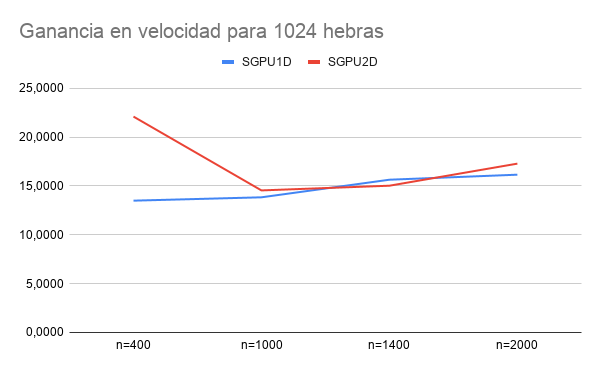
\includegraphics[scale=0.5]{img/g1024}
\end{center}

% Please add the following required packages to your document preamble:
% \usepackage[table,xcdraw]{xcolor}
% If you use beamer only pass "xcolor=table" option, i.e. \documentclass[xcolor=table]{beamer}
\begin{table}[H]
	\centering
	\begin{tabular}{|l|l|l|l|l|l|}
		\hline
		& \cellcolor[HTML]{ECF4FF}TCPU (sec) & \cellcolor[HTML]{ECF4FF}TGPU1D & \cellcolor[HTML]{ECF4FF}SGPU1D & \cellcolor[HTML]{ECF4FF}TCPU2D & \cellcolor[HTML]{ECF4FF}SGPU2D \\ \hline
		\cellcolor[HTML]{FFFFC7}n=400  & 0.162956                           & 0.011781                       & 13.8321                        & 0.00778389                     & 20.935                         \\ \hline
		\cellcolor[HTML]{FFFFC7}n=1000 & 2.52814                            & 0.161246                       & 15.6788                        & 0.143973                       & 17.5598                        \\ \hline
		\cellcolor[HTML]{FFFFC7}n=1400 & 6.92317                            & 0.406848                       & 17.0166                        & 0.418519                       & 16.5421                        \\ \hline
		\cellcolor[HTML]{FFFFC7}n=2000 & 21.5247                            & 1.11971                        & 19.2234                        & 1.02984                        & 20.9009                        \\ \hline
	\end{tabular}
	\caption{Resultados para 256 hebras}
\end{table}

\begin{center}
	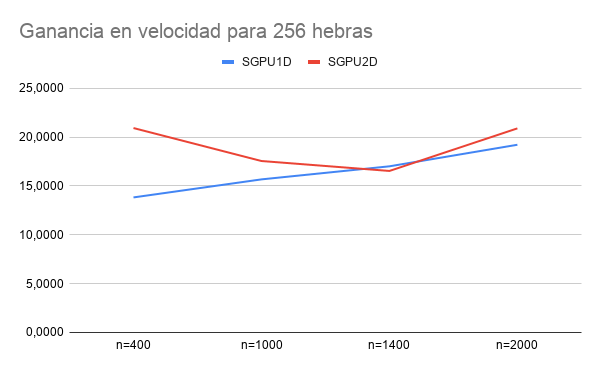
\includegraphics[scale=0.5]{img/g256}
\end{center}

% Please add the following required packages to your document preamble:
% \usepackage[table,xcdraw]{xcolor}
% If you use beamer only pass "xcolor=table" option, i.e. \documentclass[xcolor=table]{beamer}
\begin{table}[H]
	\centering
	\begin{tabular}{|l|l|l|l|l|l|}
		\hline
		& \cellcolor[HTML]{ECF4FF}TCPU (sec) & \cellcolor[HTML]{ECF4FF}TGPU1D & \cellcolor[HTML]{ECF4FF}SGPU1D & \cellcolor[HTML]{ECF4FF}TGPU2D & \cellcolor[HTML]{ECF4FF}SGPU2D \\ \hline
		\cellcolor[HTML]{FFFFC7}n=400  & 0.165771                           & 0.012486                       & 13.2766                        & 0.0127211                      & 13.0312                        \\ \hline
		\cellcolor[HTML]{FFFFC7}n=1000 & 2.62056                            & 0.160421                       & 16.3355                        & 0.289924                       & 9.03878                        \\ \hline
		\cellcolor[HTML]{FFFFC7}n=1400 & 7.63271                            & 0.391622                       & 19.49                          & 1.03841                        & 7.35039                        \\ \hline
		\cellcolor[HTML]{FFFFC7}n=2000 & 21.7567                            & 1.14077                        & 19.072                         & 2.84121                        & 7.65755                        \\ \hline
	\end{tabular}
	\caption{Resultados para 64 hebras}
\end{table}

\begin{center}
	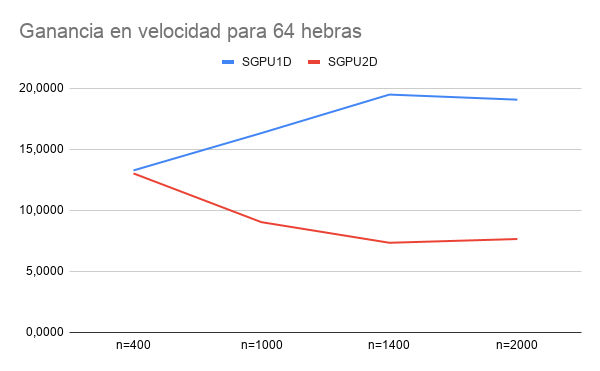
\includegraphics[scale=0.5]{img/g64}
\end{center}

% Please add the following required packages to your document preamble:
% \usepackage[table,xcdraw]{xcolor}
% If you use beamer only pass "xcolor=table" option, i.e. \documentclass[xcolor=table]{beamer}
\begin{table}[H]
	\centering
	\begin{tabular}{|l|l|l|l|l|l|}
		\hline
		& \cellcolor[HTML]{ECF4FF}TCPU (sec) & \cellcolor[HTML]{ECF4FF}TGPU1D & \cellcolor[HTML]{ECF4FF}SGPU1D & \cellcolor[HTML]{ECF4FF}TGPU2D & \cellcolor[HTML]{ECF4FF}SGPU2D \\ \hline
		\cellcolor[HTML]{FFFFC7}n=400  & 0.177634                           & 0.0277729                      & 6.39595                        & 0.029027                       & 6.11962                        \\ \hline
		\cellcolor[HTML]{FFFFC7}n=1000 & 2.62357                            & 0.404674                       & 6.48318                        & 0.429533                       & 6.10797                        \\ \hline
		\cellcolor[HTML]{FFFFC7}n=1400 & 7.78128                            & 1.08308                        & 7.18442                        & 1.18028                        & 6.59276                        \\ \hline
		\cellcolor[HTML]{FFFFC7}n=2000 & 21.6381                            & 3.11837                        & 6.9389                         & 3.28743                        & 6.58207                        \\ \hline
	\end{tabular}
	\caption{Resultados para 16 hebras}
\end{table}

\begin{center}
	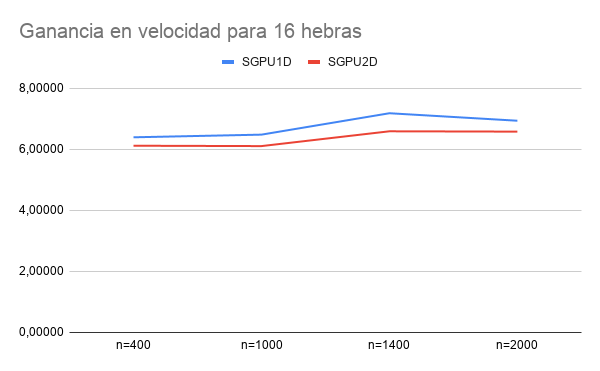
\includegraphics[scale=0.5]{img/g16}
\end{center}

Los resultados indican que la versión bidimensional obtiene mejores resultados con bloques de gran tamaño mientras que la versión unidimensional mantiene un mejor rendimiento con tamaños pequeños de bloque, a excepción de 16 hebras donde el rendimiento es bastante bajo para ambas versiones. Como ya se dijo en clase, CUDA no está pensado para ejecutarse con pocas hebras.

\subsection{Reducción para camino más largo}
Para la última parte de este ejercicio, se pide obtener la longitud del camino de mayor longitud dentro de los caminos más cortos encontrados. He utilizado una de las reducciones proporcionadas por NVIDIA en los \textit{CUDA Samples}. La reducción que ellos proporcionaban era para realizar una suma. Por tanto tuve que modificar la sección donde se realiza la suma para que buscara el máximo. El código final de la reducción es el siguiente:

\begin{minted}[bgcolor=bg,showspaces=false,breaklines=true,tabsize=4]{cuda}
template <class T>
__global__ void reduce2(T *g_idata, T *g_odata, unsigned int n) {
	// Handle to thread block group
	cg::thread_block cta = cg::this_thread_block();
	T *sdata = SharedMemory<T>();
	
	// load shared mem
	unsigned int tid = threadIdx.x;
	unsigned int i = blockIdx.x * blockDim.x + threadIdx.x;
	
	sdata[tid] = (i < n) ? g_idata[i] : 0;
	
	cg::sync(cta);
	
	// do reduction in shared mem
	for (unsigned int s = blockDim.x / 2; s > 0; s >>= 1) {
		if (tid < s) {
			if(sdata[tid] < sdata[tid+s])
			sdata[tid] = sdata[tid+s];
		}
		
		cg::sync(cta);
	}
	
	// write result for this block to global mem
	if (tid == 0) g_odata[blockIdx.x] = sdata[0];
}
\end{minted}

Hay que tener en cuenta que esta versión utiliza \textit{templates} para el tipo del conjunto de datos a operar, por tanto hay que indicar en la llamada al \textit{kernel} el tipo de dato:

\begin{minted}[bgcolor=bg,showspaces=false,breaklines=true,tabsize=4]{cuda}
reduce2<int><<<64,256,smemSize>>>(d_idata,d_odata,size);
\end{minted}

\section{Implementación CUDA de una operación vectorial}
Tanto para la versión con memoria global como para la versión con memoria compartida he optado por mantener en \textit{kernels} separados las reducciones necesarias para obtener los resultados del vector D y el máximo.

El kernel para realizar una reducción con la operación suma y así obtener el resultado de D es el mismo que utilicé en los ejercicios de CUDA. Es importante mencionar que la última reducción no se realiza en este \textit{kernel}, se realiza en la CPU. El \textit{kernel} es el siguiente: 
\begin{minted}[bgcolor=bg,showspaces=false,breaklines=true,tabsize=4]{cuda}
__global__ void reduceSum(float *d_V, float*d_out,int N){
	extern __shared__ float sdata[];
	int tid = threadIdx.x;
	int i = blockIdx.x * blockDim.x + threadIdx.x;
	
	sdata[tid] = ((i < N) ? d_V[i] : 0.f);
	__syncthreads();
	
	for (int s=blockDim.x/2;s>0;s>>=1){
		if(tid<s)
		sdata[tid] += sdata[tid + s];
		
		__syncthreads();
	}
	
	if (tid == 0)
	d_out[blockIdx.x] = sdata[0];
	
}
\end{minted}

Con respecto al kernel para buscar el máximo he utilizado el mismo que en la primera parte de esta práctica: 

\begin{minted}[bgcolor=bg,showspaces=false,breaklines=true,tabsize=4]{cuda}
template <class T>
__global__ void reduceMax(T *g_idata, T *g_odata, unsigned int n) {
	// Handle to thread block group
	cg::thread_block cta = cg::this_thread_block();
	T *sdata = SharedMemory<T>();
	
	// load shared mem
	unsigned int tid = threadIdx.x;
	unsigned int i = blockIdx.x * blockDim.x + threadIdx.x;
	
	sdata[tid] = (i < n) ? g_idata[i] : 0;
	
	cg::sync(cta);
	
	// do reduction in shared mem
	for (unsigned int s = blockDim.x / 2; s > 0; s >>= 1) {
		if (tid < s) {
			if(sdata[tid] < sdata[tid+s])
			sdata[tid] = sdata[tid+s];
		}
		
		cg::sync(cta);
	}
	
	// write result for this block to global mem
	if (tid == 0) g_odata[blockIdx.x] = sdata[0];
}
\end{minted}

Mostrados los kernels comunes a ambas soluciones, ahora solo queda mostrar las soluciones en sí. El siguiente kernel corresponde a la solución con memoria global:

\begin{minted}[bgcolor=bg,showspaces=false,breaklines=true,tabsize=4]{cuda}
__global__ void transformacion(float *A, float *B, float *C, float *D){
	int tid    = threadIdx.x;
	int i      = blockIdx.x * blockDim.x + threadIdx.x;
	int istart = blockIdx.x*blockDim.x;
	int iend   = istart + blockDim.x;
	
	C[i] = 0.0;
	
	for(int s=istart; s<iend;s++){
		float a = A[s]*i;
		
		if((int)ceil(a) % 2 == 0)
		C[i]+= a + B[s];
		else
		C[i]+= a - B[s];
	}
	
	if (tid == 0)
	D[blockIdx.x] = C[i];
}
\end{minted}

La solución con memoria compartida es la siguiente:

\begin{minted}[bgcolor=bg,showspaces=false,breaklines=true,tabsize=4]{cuda}
__global__ void transformacion_s(float *A, float *B, float *C, float *D){
	// sólo se puede utilizar 1 vector en memoria compartida
	// por tanto es necesario almacenar A,B y C en el mismo vector
	extern __shared__ float sdata[];
	float *sdata_A = sdata;
	float *sdata_B = sdata + blockDim.x;
	float *sdata_C = sdata + blockDim.x*2;
	
	int tid    = threadIdx.x;
	int i      = blockIdx.x * blockDim.x + threadIdx.x;
	
	sdata_A[tid] = A[i];
	sdata_B[tid] = B[i];
	sdata_C[tid] = 0.0;
	__syncthreads();
	
	for(int s=0; s<blockDim.x;s++){
		float a = sdata_A[s]*i;
		
		if((int)ceil(a) % 2 == 0)
		sdata_C[tid]+= a + sdata_B[s];
		else
		sdata_C[tid]+= a - sdata_B[s];
	}
	
	C[i] = sdata_C[tid];
	
	if (tid == 0)
	D[blockIdx.x] = sdata_C[tid];
}
\end{minted}

\subsection{Resultados obtenidos}
A continuación muestro una tabla con los resultados obtenidos con 32768 bloques y tamaños de bloque 64,128 y 256:

% Please add the following required packages to your document preamble:
% \usepackage[table,xcdraw]{xcolor}
% If you use beamer only pass "xcolor=table" option, i.e. \documentclass[xcolor=table]{beamer}
\begin{table}[H]
	\centering
	\begin{tabular}{|l|l|l|l|l|l|}
		\hline
		& \cellcolor[HTML]{ECF4FF}TCPU (sec) & \cellcolor[HTML]{ECF4FF}TGPU global & \cellcolor[HTML]{ECF4FF}SGPU global & \cellcolor[HTML]{ECF4FF}TGPU shared & \cellcolor[HTML]{ECF4FF}SGPU shared \\ \hline
		\cellcolor[HTML]{FFFFC7}64  & 0.521583                           & 0.0126719                           & 41.1605                             & 0.011178                            & 46.6615                             \\ \hline
		\cellcolor[HTML]{FFFFC7}128 & 2.04164                            & 0.0357029                           & 57.1841                             & 0.0292981                           & 69.6851                             \\ \hline
		\cellcolor[HTML]{FFFFC7}256 & 7.89317                            & 0.119995                            & 65.7793                             & 0.072989                            & 108.142                             \\ \hline
	\end{tabular}
\end{table}

Como se puede ver, la versión con memoria compartida es superior al resto; siendo las versiones de GPU muy superiores a la versión de CPU.
Para finalizar me gustaría añadir que los kernels que realizan las reducciones se podrían lanzar simultaneamente, consiguiendo aún mas eficiencia.

A continuación muestro las comparaciones en formato gráfico:

\begin{center}
	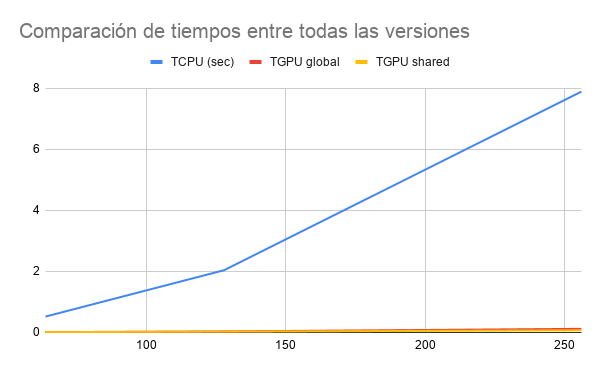
\includegraphics[scale=0.5]{img/compall}
\end{center}

\begin{center}
	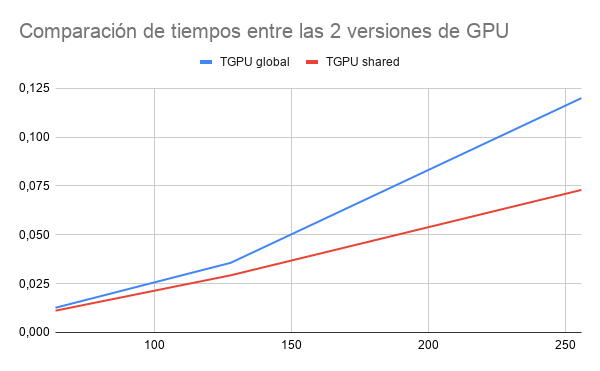
\includegraphics[scale=0.5]{img/compt2}
\end{center}

\begin{center}
	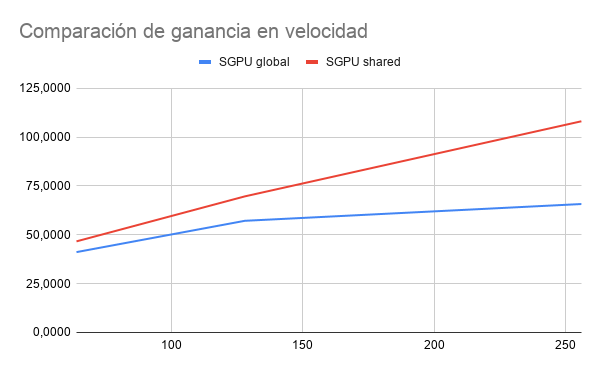
\includegraphics[scale=0.5]{img/comps2}
\end{center}



Todo el código aquí mostrado se incluye también con la entrega de la práctica junto con \textit{Makefiles} individuales.

\end{document}